\section{Datos}
\label{sec:datos}

Usamos el subconjunto público \code{hagrid-sample-30k-384p} \citep{mills_hagridsample} de HaGRID,
con imágenes de 384\,px y las anotaciones originales: la caja de cada mano, su etiqueta y un
identificador anónimo de la persona (\code{user\_id}). Elegimos los ocho gestos de la
\cref{tab:datos}, que cubren las órdenes básicas de un robot móvil con pinza. Sus
\NImagenesOrig{} imágenes contienen \NManos{} manos de \NPersonasOrig{} personas. La clase nula
está formada por las \NoGestureOrig{} \emph{segundas manos} de esas mismas imágenes, que HaGRID
etiqueta como \cls{no\_gesture} porque no hacen el gesto. Así, los negativos comparten persona,
fondo e iluminación con los positivos, y la red no puede separar las clases por el contexto. Para
equilibrar las clases, submuestreamos la nula hasta \NoGestureKept{} ejemplos, el tamaño medio de
una clase de gesto.

Cada mano se recorta como un cuadrado centrado en su caja, de lado 1,5 veces el lado mayor de la
caja (un margen del 25\,\% por cada lado), y se redimensiona a $128\times128$\,px
(\cref{fig:recortes}). Las manos son pequeñas (la mediana del lado de la caja es de
\LadoCajaMediana), así que la mayoría de los recortes se amplían.

La partición usa \code{StratifiedGroupKFold} con \code{user\_id} como grupo: 20 trozos
estratificados por clase, de los que 14 van a entrenamiento, 3 a validación y 3 a test
(70/15/15). Resultan \NTrain{}, \NVal{} y \NTest{} recortes de \PersonasTrain{}, \PersonasVal{} y
\PersonasTest{} personas, sin ninguna persona compartida entre particiones (lo comprueba una
prueba automática). La normalización por canal usa estadísticas calculadas solo con
entrenamiento.

\begin{table}[t]
  \centering
  \caption{Vocabulario de órdenes y recortes por clase y partición, tras equilibrar
    \cls{no\_gesture}. Ninguna persona aparece en más de una partición.}
  \label{tab:datos}
  \small
  \TablaDatos
\end{table}

\begin{figure}[t]
  \centering
  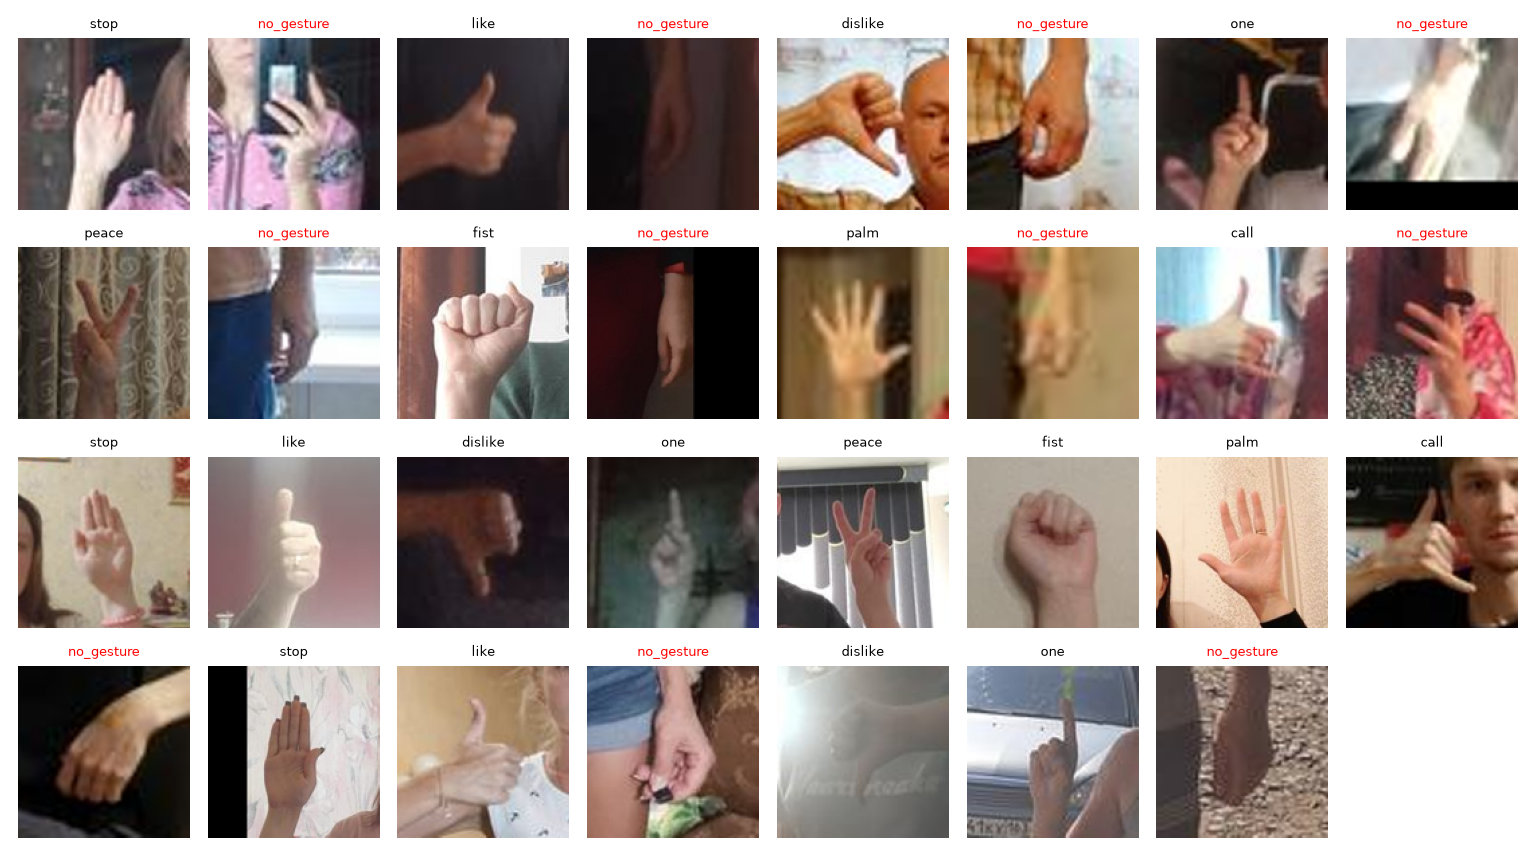
\includegraphics[width=0.8\linewidth]{figures/recortes_muestra.png}
  \caption{Recortes de $128\times128$\,px de las nueve clases. Los de \cls{no\_gesture} (en rojo)
    son manos en reposo, sujetando objetos o parcialmente visibles.}
  \label{fig:recortes}
\end{figure}
